\documentclass{kththesis}

\usepackage{textcomp}
\usepackage{lmodern}
\usepackage{amsmath}
\usepackage{amsfonts}
\usepackage{amssymb}
\usepackage{amsthm}
\usepackage{color}
\usepackage{graphicx}
\usepackage{hyperref}
\usepackage[ruled,vlined]{algorithm2e}
\newtheorem{thm}{Theorem}
\definecolor{gris25}{gray}{0.95}
\newcommand{\encadre}[1]{\hspace{-20pt}\fcolorbox{black}{white}{\begin{minipage}{0.99\textwidth}\medskip #1 \vspace{5pt}\end{minipage}}\bigskip}
\newtheorem{prop}[thm]{Property}
\newtheorem{lem}[thm]{Lemme}
\newtheorem{cor}[thm]{Corollaire}
\newtheorem{hyp}[thm]{Hypothesis}
\def\N{{\mathbb{N}}}
\def\R{{\mathcal{R}}}
\def\P{{\mathbb{P}}}
\newcommand\independent{\protect\mathpalette{\protect\independenT}{\perp}}
\def\independenT#1#2{\mathrel{\rlap{$#1#2$}\mkern2mu{#1#2}}}


\usepackage{csquotes} % Recommended by biblatex
\usepackage[style=ieee,backend=bibtex]{biblatex}
\addbibresource{../Specs/specifications_ref.bib} % The file containing our references, in BibTeX format


\title{Estimating the probability of event occurrence}
\alttitle{Uppskattning av sannolikheten för händelse} %TODO
\author{Alexandre GUINAUDEAU}
\email{alegui@kth.se}
\supervisor{Pawel Herman}
\examiner{Hedvig Kjellstr{\"o}m}
\programme{Master in Computer Science}
\school{School of Electrical Engineering and Computer Science}
\date{\today}

\tolerance=1600

\begin{document}

% Frontmatter includes the titlepage, abstracts and table-of-contents
\frontmatter

\titlepage

\begin{abstract}
%TODO
  English abstract goes here.

\end{abstract}


\begin{otherlanguage}{swedish}
  \begin{abstract}
  %TODO
    \emph{I will translate my abstract once the English version has been approved.}
  \end{abstract}
\end{otherlanguage}


\tableofcontents


% Mainmatter is where the actual contents of the thesis goes
\mainmatter

%\chapter{Introduction}
%
%\section{Research Question}
%
%\chapter{Methods}


\chapter*{Introduction}

In complex systems, errors can occur intermittently and in a non-deterministic way, which makes it harder to diagnose real errors among spurious ones. 
In manufacturing for instance, intermittent errors could be due to physical properties, either internal, like bad contacts, or external, e.g. extreme temperatures.
In any case, these errors are often hard to troubleshoot and require close attention. By analogy with \emph{flaky tests} in computer science, we will also refer to these as \emph{flaky errors}.\\

Non-deterministic errors are often considered as unreliable and therefore discarded, which creates an important risk of ignoring a real error. On the other hand, troubleshooting each occurrence of a flaky error is very time-consuming and is not always an option. Therefore, it is critical to detect when flaky errors occur at an unexpected rate and to pinpoint when the rate of failure is likely to have evolved. This enables engineers to understand which elements have an impact on the error. In computer science, the usual workaround for flaky tests is to re-run tests that failed a certain number of times until they pass. In other fields, this is not always possible as errors are triggered in a production environment.\\

In this thesis, we intend to estimate the underlying probability of occurrence of an error.
We assume its distribution to be piecewise
stationary. This corresponds to the fact that the probability of
occurrence changes when a part breaks, wears out, or is repaired. Given this assumption, estimating the underlying probability of occurrence is
equivalent to finding its change points.

\clearpage

\chapter{Pilot study}

\section{Objective}

Given a sequence of events, we intend to detect changes in the probability of occurrence. This has two main interests:

\begin{itemize}
\item Alert when events start occurring more frequently.
\item Troubleshoot errors by pinpointing when the probability of occurrence changed.
\end{itemize}

For instance, in the case of intermittent errors due to bad contact, the detection of change in frequency could enable users to understand that high vibrations triggered the bad contact, and that some specific maintenance work fixed it.

According to \parencite{baigneres2004}, two binomial distributions $Bin(n, p)$ and $Bin(n, p+\varepsilon)$ (where $n$ is the number of observations, and $p \gg \varepsilon$ the probability of occurrence of the event) can be distinguished after 
$$n \sim \dfrac{K}{\varepsilon^2}$$
observations, for some $K$ independent of $\varepsilon$.
So a change in probability of $0.1$ should be detected within the order of $n \sim 100$ observations.


\paragraph{News value}

In complex systems, it may be too time-consuming to monitor all the errors that occur. in that case, unusual errors are carefully troubleshooted, but intermittent and non-deterministic errors can end up being ignored. In that case, being able to flag when an error occurs more frequently than usual can be vital. Indicating precisely when the frequency increased significantly is also very useful to quickly understand the reason for this increase in frequency and troubleshoot the error.

\section{Research question}

\textbf{What is the sensitivity of detection of changes in the frequency of event occurrence? In other words, given a target level of confidence, what is the minimum change in the frequency that can be identified, and what delay is necessary to reliably identify this change?}

\medskip

\paragraph*{Examination method}

First, we will find the tuning of the parameters both candidate models that provide the target confidence level. 
Therefore, we will use the mathematical definition to estimate the how the parameters should be tuned, and we will approximate the actual parameters using Monte Carlo methods. 

Then, we will compare the sensitivity and delay of the models. We will generate data with a single change point, and measure the number of observations required to detect the change, depending on the amplitude of the change.

Finally, we will discuss how well both models could be generalized to real data. 
To emulate real data do so, we will generate sequences of probabilities of occurrence in a \emph{realistic} way (See \ref{part-lifetime}), and derive events based on those probabilities. Then, we will estimate the underlying probabilities based on the events, and compare the candidate models to find the one that performs best. We will also compare efficiency of the algorithms (in terms of memory and computation), and see how easily they could be adapted to online data.

\paragraph*{Expected scientific results}

The hypothesis being tested is that we are able to detect \emph{significant} changes in probability of occurrence, \emph{shortly} after the change. 
The only parameter of our model should be the target level of confidence (for instance $95\%$).
Performing maintenance is usually very expensive as it often requires to replace a part. Therefore, we only want to trigger an alert if we have sufficiently high  confidence that a change in the frequency actually occurred.

Given these, we want to measure:

\begin{itemize}

\item the \emph{sensitivity} of the detection: the minimal increase or decrease in the frequency of occurrence that we are able to detect
\item the \emph{delay} of the detection: the minimal number of observations after a change in frequency required to detect a change

\end{itemize}

To measure the accuracy of our estimations, we will compare their sensitivity and delay on generated data with a single change point.

For data with multiple change points, we would use the $\mathcal{L}_2$ score to measure the error with the true underlying distribution.

\section{Literature study}

\paragraph{Generating events}
\label{part-lifetime}

To generate our data, we will simulate part failures that lead to an increased probability of triggered events. Interestingly, the lifetime of organisms, devices, structures, materials in both biological and engineering sciences have very similar behaviors. 
For example, business mortality \parencite{lomax1954}, failures in the air-conditioning equipment of aircrafts or in semiconductors \parencite{proschan1963} and integrated circuit modules \parencite{saunders1983} all have similar behaviors. 
These can be modeled with a mixture of exponential or Weibull-Lomax distributions. In particular, the Weibull distribution \parencite{weibull1951} is the most widely used to model the lifetime of parts \parencite{anderson2005}, as it has a limited number of parameters which can easily be interpreted, and captures both the \emph{infant mortality} of defective parts and the exponential distribution of events that occur independently at a constant average rate, for normal parts. The two parameters are used to reflect these two elements, the defects in the material and the average rate of failure.

\paragraph{Detection of probability change-points}

The detection of a change point can be formulated as a null hypothesis that determines whether all events were drawn from the same binomial distribution \parencite{wasserman2004}.
To generalize this to multiple change points, we could use a sliding window. However, this is often unstable because the change point detection is performed on small regions, and therefore isn't always statistically significant \parencite{esteller2001, harchaoui2010}.
Therefore, we will also explore binary segmentation or dynamic programming to generalize our algorithm to sequences of events with multiple change points \parencite{jackson2005}, while still running in linear time \parencite{killick2012}.


Another lead could be to use Hidden Markov Models \parencite{baum1966}, which seems well-adapted to our use case, as we are trying to guess the hidden probability state that was used to generate the events. Chis and Harrison \parencite{chis2015} suggest a solution to adapt the model to online problems by estimating its updated parameters. This can be used to avoid recomputing the hidden state with new values.


\section{Specific problem definition}

\paragraph{Definitions}

As we will generate our data, it is important to clearly specify how the data is generated and what assumptions are made.

We consider a complex system composed of many different physical parts, and equipped with a logging system that triggers an error when an unusual behavior is detected. 
This logging system stores a sequence of observations $t$, for which events either occurred or did not.
These observations could be of various time scales, either periodic (e.g. 1 per second) or based on iterations (e.g. one per cycle in manufacturing). 
We consider a single event $e$, independently of the other ones that were recorded by the logging system.

\begin{itemize}
\item We call \emph{observation} $t$ each iteration where a value is stored by the logger.

\item We call \emph{event} or \emph{error} $e$ a specific kind of event that was recorded by a logging system. For each observation $t$, we note $y_t=1$ if the event occurred and $y_t=0$ otherwise. We note $p(t)=\P[y_t=1]$ the probability that $e$ occurs at instant $t$.

\item We call \emph{part} a physical part of our system; it can be anything from a valve to a sensor. The failure or wear of such a part could increase the probability of occurrence of $e$, and maintenance or replacement of the part could decrease it.

\item We call \emph{change point} any of these changes affecting a part which has an impact on $e$.
\end{itemize}

\paragraph{Assumptions}

We assume that the event occurs with a fixed probability $p$, independent of previous events, between two consecutive change points. 
Note that this is not a lost in generality intrinsically, given we could consider change points at every observation. However, we will in general consider a low frequency of change points.

To tune the parameters of our models, we will consider events generated with a constant probability $p$. 
To evaluate their sensitivity and delay, we will consider events generated with to probabilities $p_1$ and $p_2$, and a single change point.
To evaluate their capacity to generate to real-life data, we will use a Weibull distribution to model the lifetime of parts, and derive series from successive underlying probabilities.

\section{Using a null hypothesis to tune our models}

As mentioned earlier, we want to define models with a single parameter, the target level of confidence $\alpha$. We will tune the parameters of our models such that the probability that we erroneously detect a change point is at most $\alpha$. 
Given a sequence of events $y_0, \ldots, y_{T-1}$, we consider the null hypothesis:\\

\encadre{$H_0$: All events $y_0, \ldots, y_{T-1}$ were drawn from the same Bernoulli distribution $B(1,|y|)$}


If the model is correctly tuned, we should reject this null hypothesis with a probability of $\alpha$ for distributions drawn from a constant distribution. Therefore, when our model detects a change point, we can assert that the underlying probability of occurrence has changed with a confidence of $1-\alpha$.

\chapter{Hidden Markov Model}

\section{Mathematical definition}
\label{sec:hmm_math_definition}

The first model we consider to estimate the underlying probabilities is a Hidden Markov Model, where the hidden states are the underlying probabilities.

We note $x_t$ the hidden state at $t$ and $y_t$ the corresponding observation. The parameters of a HMM are:

\begin{itemize}
\item The number of states $N$. In our case states correspond to probabilities $p_0, \ldots, p_{N-1}$
\item The number of observations $T$, observations are noted $y_0, \ldots, y_{T-1}$
\item The initial hidden state $\varphi_i = \P[x_0=p_i]$
\item The transition probabilities $\phi_{i,j} = \P[x_{t+1}=p_j\ |\ x_t = p_i]$
\item The distribution from which observations are drawn. Here, observations are drawn from a Bernoulli distribution: $y_t \sim B(1, x_t)$
\end{itemize}

Given $N$, there are $\mathcal{O}(N^2)$ independent parameters $\varphi_i$ and $\phi_{i,j}$. We will make a few additional assumptions to reduce the complexity. 

\paragraph{Uniformly distributed states}
We assume the states are uniformly distributed on the interval $[0, 1]$:
$$\forall i \in [|0, N-1|], p_i = \dfrac{i}{N-1}$$
This is not a loss in generality, as we can increase the number of states to cover any possible probability $p \in [0,1]$

\paragraph{Uniform prior distribution}
No particular prior distribution is assumed, so the initial states are sampled from a discrete uniform distribution over all possible states:

$$\forall i \in [|0, N-1|], \varphi_i = \dfrac{1}{N}$$

\paragraph{Uniform change amplitude}
We also assume that when a change occurs, all new states are equiprobable, in other words that, given $i$, $\phi_{i,j}$ is constant for any $j \neq i$. 

\paragraph{Uniform change likelihood}
We also assume that probability that a change occurs is independent of the current state, in other words that $\phi_{i,i}$ is constant. This assumption is more debatable, as when errors occur frequently, operators are likely to do maintenance operations that will decrease the frequency of occurrence. For the sake of simplicity, we will make this assumption for now and discuss this choice in the later (See \ref{chap: discussion}).

With these two assumptions on $\phi$, the matrix of transition probabilities now has two values, one for diagonal coefficients $\phi_{i,i}$ and one for extra-diagonal coefficients $\phi_{i,j}$. We note $\rho$ the ratio between these two coefficients:

$$\rho = \dfrac{\phi_{0,1}}{\phi_{0,0}}$$

As for each row, the sum of its coefficients is 1, we can derive the value of all the transition probabilities from $\rho$:

$$
\phi_{i,j} = \left\{
\begin{array}{ll}
\dfrac{1}{1 + (N-1) \rho} & \text{if } i = j  \\
&\\
\dfrac{\rho}{1 + (N-1) \rho} & \text{if } i \neq j
 \end{array}\right.
$$

With these assumptions, we have reduced the complexity of our model to a single parameter $\rho$. In the next section, we will find the best value of $\rho$ given the number of states $N$, the number of observations $T$, the probability of occurrence $p$ and the target level of confidence $\alpha$.

\section{Tuning the Hidden Markov Model}

The Baum-Weich algorithm \parencite{baum1966} provides the most likely set of underlying probabilities, given the parameters of the model and a sequence of observations.
We will use this algorithm to detect change points, when the most probable state contains at least two different states.

\section{Mathematical interpretation}

\paragraph{Influence of $\rho$ on the detection of change points}
Our Hidden Markov Model has been reduced to a single parameter $\rho$. It important to first understand how this parameter will impact the behavior of the HMM. When $\rho$ increases, the relative probability of changing state increases, so the HMM is more likely to detect a change point. 
Our goal is to find the maximum value of $\rho$ that detects a change point with a probability at most $\alpha$.

\paragraph{Influence of $N$ on $\rho$}
To determine the most likely sequence of underlying states, the Baum-Weich algorithm does a forward pass during which it computes the most likely state up to the current observation, and then a backward pass where it updates the likelihoods that could have lead to the final state. 

This can be seen as a trade-off between two opposite "energies": changing the underlying state from $i$ to $j$ costs $\mathcal{E}_{i \rightarrow j} \sim \frac{\phi_{i,j}}{\phi_{i,i}}$, while staying in the current state $i$ costs $\mathcal{E}_{i \not\rightarrow j} \sim \frac{\overline{p_i}}{\overline{p_j}}$ where $\overline{p_k}$ represents the probability of predicting the wrong state ($1-p_k$ if the even occurred, $p_k$ otherwise). The Baum-Weich algorithms finds the sequence of states that minimizes this energy: it is only worth changing state if many future observations are very unlikely the current state $i$. 

Using our assumptions in \ref{sec:hmm_math_definition}, these energies become $\mathcal{E}_{i \rightarrow j} \sim \rho$ and $\mathcal{E}_{i \not\rightarrow j} \sim \frac{\overline{p_i}}{\overline{p_j}}$.
Note that these energies are now independent of $N$: the only impact is that, for small values of $N$, all probabilities $p_i$ and $p_j$ will not be represented. In other words, there might not be the state corresponding to the actual underlying probability. However, for sufficient large value of $N$, $\rho$ is independent of $N$.
 
The choice of $\rho$ as the single parameter to tune the model was not arbitrary: it is independent on the number of states $N$. Figure \ref{fig:hmm_nstates_rho} shows an example using Monte Carlo method with $n_{tries}=1000$ tries, where we approximate the optimal $\rho$ with a precision of $0.001$. In the rest of this report, we will use $N=101$ states, so that the states represent $0\%, 1\%, 2\%, \ldots, 100\%$.

\begin{figure}[ht]
\hspace{-50pt}
\includegraphics[width=1.25\textwidth]{images/hmm_nstates_rho}
\caption[caption]{Maximum transition probability ratio $\rho$ that does not detect a change point, for different levels of confidence $\alpha$\\
For $p = 20\%$, $T = 100$, $n_{tries} = 1000$, $precision=0.001$}
\label{fig:hmm_nstates_rho}
\end{figure}


\paragraph{Influence of $\alpha$ on $\rho$}

We expect $\rho$ to be an increasing function of the level of confidence $\alpha$: if we loosen our restrictions and accept a higher risk of erroneously detecting a change, then we can increase the transition probability ratio. When plotting some examples \ref{fig:hmm_alpha_rho}, it seems clear that for small values of $\alpha$, there is a linear correlation between $\alpha$ and $\rho$.

\begin{figure}[ht]
\hspace{-50pt}
\includegraphics[width=1.25\textwidth]{images/hmm_alpha_rho}
\caption[caption]{Maximum transition probability ratio $\rho$ that does not detect a change point, for different probabilities of occurrence $p$\\
For $N = 101$, $T = 100$, $n_{tries} = 1000$, $precision=0.001$}
\label{fig:hmm_alpha_rho}
\end{figure}

\subsection{Application to events derived from a constant probability}

\subsection{Detection of a single change point}



\chapter{Binary Segmentation Model}



\chapter{Model comparison and Discussion}
\label{chap: discussion}
%TODO Discuss a more complex HMM

\section{Detection of single change points}

\section{Generalization to multiple change points}

\section{Efficiency and generalization to an online algorithm}


\chapter{Conclusion}

\section{Discussion}

\section{Future Work}

\printbibliography[heading=bibintoc]

\end{document}

%%%%%%% OLD VERSION OF THE REPORT %%%%%%%%
%
%As it spreads to many industries and increases in volume, sensor data is a becoming an important field of research in terms of security, storage, and analysis.
%In manufacturing plants, aircrafts, electronic intensive care units or data centers, sensors continuously monitor many parameters of the environment.
%The data generated by these sensors is then processed to optimize the way the system works, or to diagnose failures once they occurred.
%These systems can have hundreds or thousands of sensors with sub-second sampling.
%With this amount of data, diagnosing failures requires an efficient processing of the data.\\
%
%Finding other data that is associated with the failures and can contribute to explaining them is critical to understand the circumstances of the incident and troubleshoot it.
%In most cases, the cause of the failures is specific to what the data represents.
%For instance, the sensor data could be a consequence of the failure rather than a cause, or a third factor could have affected both the sensor and the system.
%In any case, providing the system engineer with a limited list of sensors that seem to have some correlation with the failure is very valuable to enable them to quickly troubleshoot the problem.
%Once the engineers know where to look, they are usually able to understand what happened by diving into the specific environment parameters.
%
%\clearpage
%
%\chapter{Pilot study}
%
%\section{News value}
%
%Automatically finding associated sensor time series would be very valuable for all of the systems described above to troubleshoot failures faster and anticipate them. 
%It could be applied to any system that has a logging system generating frequent debug messages and a few error events independently.
%Microsoft researched suggested a solution to correlate continuous and event time series \parencite{zhang2014} but focused more on the temporal correlation - so the causal correlation - rather than the actual association between timeseries. For non-stationary time series, we assume they have been transformed to be stationary - or more exactly, we will show some ways to transform stationary timeseries to stationary ones.
%
%% My thesis is motivated by a real-world application of incident diagnosis.
%
%\section{Correlation metrics}
%The most common metric to measure correlation is the \emph{Pearson} coefficient. It can easily be interpreted and visualized \parencite{rodgers1988}, and often gives very good results. However, in some case, it can be misleading, especially because it only captures linear correlations and because it assumes normal distribution of the input parameters.
%
%In this case, the \emph{Spearman} coefficient is more robust (although less efficient), as it only compares ranks between elements, and therefore captures monotonic correlations, even if there are not linear. The \emph{Kendall} coefficient is very similar as it also uses the rank of elements to compare them, it is less efficient but more robust. It is also much easier to interpret, as it captures the percentage of elements positively correlated \parencite{valz1994, xu2010}. These correlation metrics are probably more adapted to our problem for numerical data as they capture non-linear correlations, but may be harder to generalize because their definition is not as simple as Pearson's.
%
%\section{Association metrics}
%
%All these usual correlation metrics apply to numerical data, and cannot therefore be used for categorical data. In this case, a metric that often works well is the J-measure \parencite{smyth1992, goodman1992}, which is based on the concept of entropy in information theory. For binary data, it is possible to transform the data to make most association measures equivalent \parencite{tan2004}. This is not as clear for more complex data, and requires to clearly define the concept of association for categorical and continuous data as well.
%
%However, it is not clear if this measure can be compared to the previous ones when the data is both numerical and categorical - for instance when it is binary. In \parencite{tan2004}, P-N Tan et al. compared many existing norms on binary classification, and showed their was a way to normalize the data in order to make all the norms they studied equivalent. Such techniques will be important to pre-process the data accurately and to generalize norms to heterogeneous time series.
%
%\section{Application to heterogeneous data}
%Several tools exist to analyze the correlation between continuous time series \parencite{wu2010}, or between events \parencite{lou2010}, but they do not perform well when it comes to correlating continuous time series and events. However, sensor data is heterogeneous: it can be continuous, discrete, categorical or binary.
%Usual measures of correlation such as the Pearson and Spearman correlation do not perform well on this kind of data \parencite{zhang2014}.
%Therefore, we have to find other ways of defining association. We can also map continuous or categorical time series to event time series - by detecting outliers or change points - and apply existing tools to the transformed data \parencite{stoffer1993, guralnik1999}.

%\newpage
%
%\chapter{Defining association for hetero\-geneous time series}
%
%In order to find time series which can help us troubleshoot failures, we must first define \emph{association} in a clear way. 
%To do so, we will define a set of properties that a good association metric should abide by, and then define very simple examples where we know how the association metric should behave. 
%Then, we will compare candidate metrics based on these properties and examples in order to select the ones that correctly measure association.
%
%\section{Fundamental properties}
%\label{sec:properties}
%
%\subsection{Notations and definitions}
%
%Given two time series $x$ and $y$, we note $A(x, y)$ the association between them. Without loss of generality, we can assume that our metric gives a score from 0 to 1.
%$x$ and $y$ are associated if the knowledge of one improves the understanding of the other, in other words if the posterior model forecasts values better than the prior model.
%
%More formally, we note $\mathcal{P}(x_t | x_0, \ldots, x_{t-1})$ the forecast of $x_t$ at the instant $t$, given all previous observations, and $\mathcal{P}_y(x_t | x_0, \ldots, x_{t-1})$ the forecast of $x_t$ at the instant $t$ given all previous observations of $x$ and all observations of $y$.
%
%We also define a loss metric $\mathcal{L}$ which measures the surprise:
%
%$$\mathcal{L}(x)_t = dist(\mathcal{P}(x_t | x_0, \ldots, x_{t-1}), x_t)$$
%$$\mathcal{L}(x|y)_t = dist(\mathcal{P}_y(x_t | x_0, \ldots, x_{t-1}), x_t)$$
%
%where $dist$ is a distance metric. 
%
%\subsection{Properties}
%
%With these notations, a good metric to measure association between time series should follow the following properties:\\
%
%\noindent
%\fbox{
%    \parbox{\textwidth}{%
%\begin{enumerate}
%    \vspace{-.5em}
%    \item[\textbf{P1.}] \textbf{(Independence)} $A(x, y) = 0 \Leftrightarrow x \independent y$
%    \item[\textbf{P2.}] \textbf{(Information gain)} $ A(x, y) > 0 \Leftrightarrow \mathcal{L}(x | y) < \mathcal{L}(x)$
%    \item[\textbf{P3.}] \textbf{(Perfect knowledge)} $A(x, y) = 1 \Leftrightarrow \mathcal{L}(x | y) = 0$
%    \item[\textbf{P4.}] \textbf{(Symmetry)} $A(x, y) = A(y, x)$: $A$ should be symmetric
%    \vspace{-.5em}
%\end{enumerate}
%    }%
%}
%
%\section{Expected behavior for simple examples}
%\label{sec:simple_examples}
%
%We also define simple examples where we can know how the association should behave.
%
%\subsection{Categorical and event data}
%
%Our first example compares an event time series and a categorical one. This could for instance be useful to determine whether an installed part tends to fail more often than another. We will start with the case of two categories and then generalize to any number of categories.
%Let $x$ be a time series of events, that occur with probability $p_1$ during $t_1$ and then at frequency $p_2$ during $t_2$. Let $t_{tot} = t_1 + t_2$ the total time, 
%$p_{tot} = \frac{p_1 n_1 + p_2 n_2}{n_1+n_2}$ the average probability of failure. Let $y$ be a categorical time series with value $C_1$ during $t_1$ and $C_2$ during $t_2$. Figure \ref{fig:categorical_event_series} shows an example of such time series $x$ and $y$.
%
%\begin{figure}[ht]
%\centering
%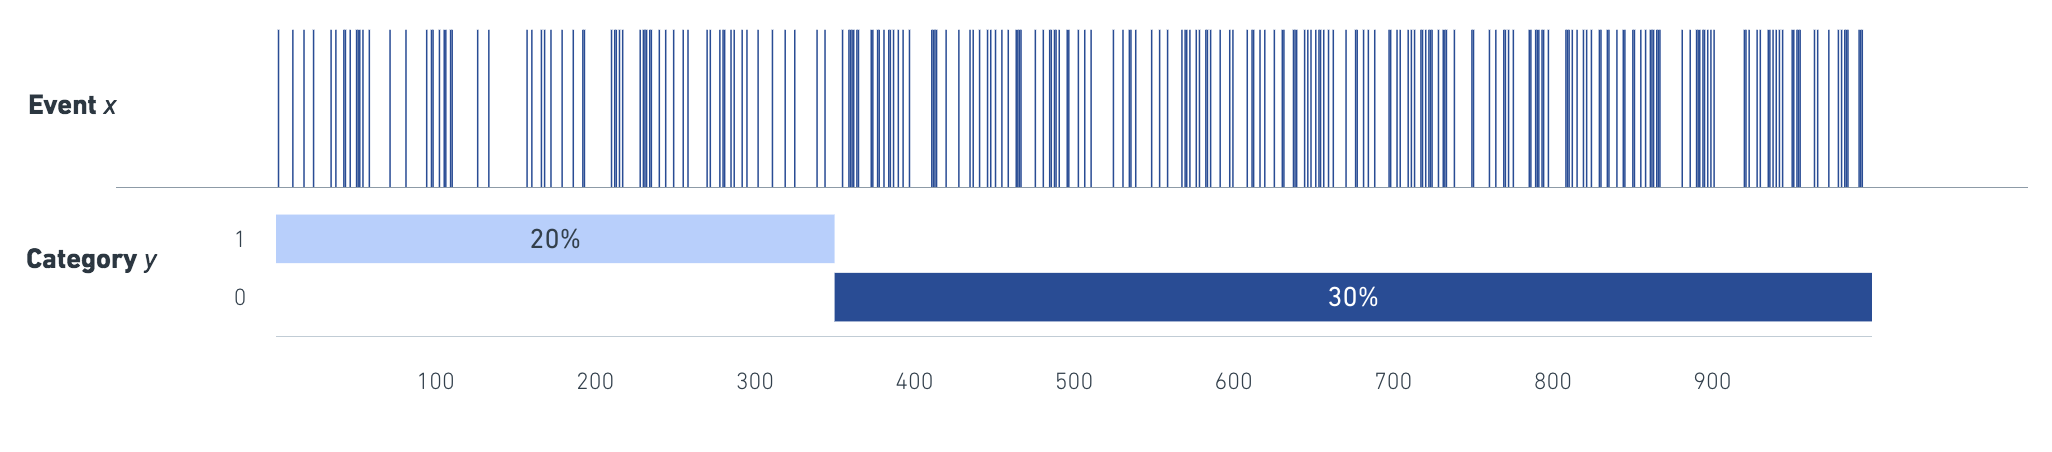
\includegraphics[width=\textwidth]{images/categorical_event_series}
%\caption[caption]{Example of associated categorical and event series\\
%For $p_1 = 20\%$, $p_2 = 30\%$, $t = 1000$, $t_1 = 350$}
%\label{fig:categorical_event_series}
%\end{figure}
%
%Let's consider other candidate time series $y_k$ with value $C_1$ during $t_1'=k$ and $C_2$ during $t_2'=t_{tot}-k$. 
%A good association metric should rank $y_i$ time series such that $y_{t_1}$ has the highest association with $x$. 
%
%\subsection{Numerical and event data}
%
%For numerical data, we cannot expect to have a metric that computes the association in the right way on any raw dataset, because the association depends on what the data represents. 
%Events can be triggered by extreme values or by sudden changes, they can depend on the original value, or on the de-trended or de-seasoned value. 
%Events could also have an impact in the future, or for a specific duration. 
%Therefore, we assume the data is preprocessed (potentially de-trended, de-seasoned, shifted, smoothed, derived, normalized) such that large values have a higher risk of triggering an event. 
%This is not a real loss of generality, because one can derive multiple preprocessed series out of the original one, for instance using all the methods described above, and the algorithm will only find candidates with high association with the event series.
%
%Let $x$ be a time series of $N$ events, and $y \sim \mathcal{N}(0, \sigma)$ be a series of Gaussian white noise, which could be for instance the residual of a de-seasoned and de-trended series. When an event occurs, $y$ has a higher value in average:
%
%$$
%y \sim \left\{
%\begin{array}{ll}
%\mathcal{N}(0, \sigma) & if\ x = 0 \\
%\mathcal{N}(1, \sigma) & if\ x = 1
% \end{array}\right.
%$$
%
%In this case, we expect $x$ and $y$ to be highly associated. Furthermore, if we define other numerical series that are impacted by a fraction of the events, or by additional events, they should have a lower association with $x$. Figure \ref{fig:numerical_event_series} shows and example of such series $x$ and $y$. 
%
%\begin{figure}[ht]
%\centering
%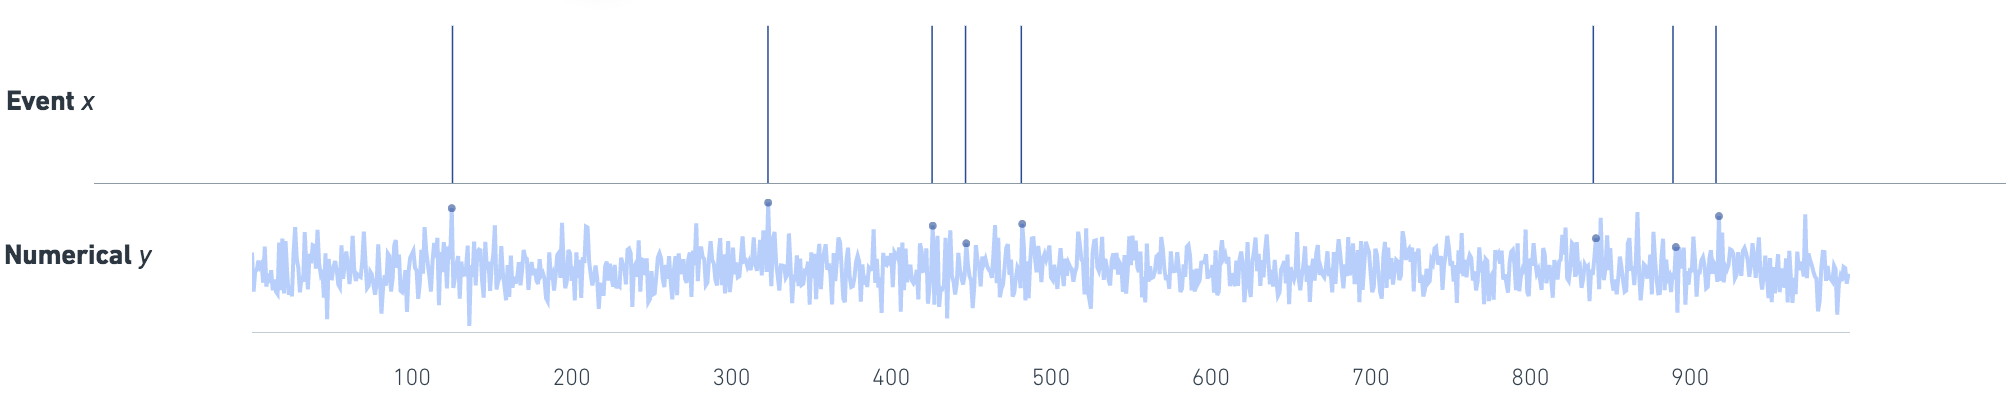
\includegraphics[width=\textwidth]{images/numerical_event_series}
%\caption[caption]{Example of associated numerical and event series\\
%For $8$ events, $\sigma = 0.4$}
%\label{fig:numerical_event_series}
%\end{figure}
%
%Let's consider other numerical time series $y_k$ having larger values for either a subset (if $k < N$) or a superset (if $k > N$) of the events $x$. 
%More precisely, we generate a series of events $x$ and note $N$ the number of events. Then, for $k \in [0, N-1]$, we define $x_k$ by selecting a subset of the events of size $k$, selected at random. For $k \in [N+1, 2N]$, we define $x_k$ composed of all the events of $x$ as well as $k-N$ other events. We note $x_N = x$.
%
%We now define $y_k$ for $k \in [0, 2N]$:
%
%$$
%y_k \sim \left\{
%\begin{array}{ll}
%\mathcal{N}(0, \sigma) & if\ x_k = 0 \\
%\mathcal{N}(1, \sigma) & if\ x_k = 1
% \end{array}\right.
%$$
%
%A good association metric should rank these time series such that $y_{k=N}$ has the highest association with $x$.
%
%
%\section{Comparison of different metrics}
%
%We will start by studying usual metrics that could capture the association between time series. We will compare them based on the properties and examples defined in sections \ref{sec:properties} and \ref{sec:simple_examples}, and see how they can be generalized to apply to any time series.
%
%\subsection{Pearson Correlation Coefficient}
%The most common measure of correlation is the one defined by Pearson $\rho$ defined by:
%
%$$
%\rho_{x,y} = \frac{cov(x, y)}{\sigma_x \sigma_y} =  \dfrac{\sum_i (x_i - \overline{x}) (y_i - \overline{y})}{\sqrt{\sum_i (x_i - \overline{x})^2} \sqrt{\sum_i (y_i - \overline{y})^2}}
%$$
%
%To capture both correlated and anti-correlated time series we consider its square value $\rho^2$. 
%
%\paragraph{Properties}
%It verifies all implications ($\Rightarrow$) of the above properties: a high Pearson correlation coefficient indicates that the knowledge of a series increases our knowledge of the other. However, it only captures linear correlation, so we could miss association between series with non-linear correlation (\textbf{P2.} $\nLeftarrow$ and \textbf{P3.} $\nLeftarrow$). 
%
%\paragraph{Categorical data}
%In order to compute the Pearson correlation coefficient for the first example, we need the categorical data to have numerical values, we set $C_1 = 1$ and $C_2 = 0$.
%
%Figure \ref{fig:categorical_pearson} displays the squared Pearson correlation coefficient $\rho_{x,y_k}$ for values of $t_1' = k$ from $0$ to $t$. 
%In this example, the largest Pearson correlation coefficient is reached for $t_1'^* = 999$. If we ignore this edge case, the second largest value of $t_1'$ with highest score is $320$, which is close to the optimal value $t_1 = 350$. 
%
%\begin{figure}[ht]
%\centering
%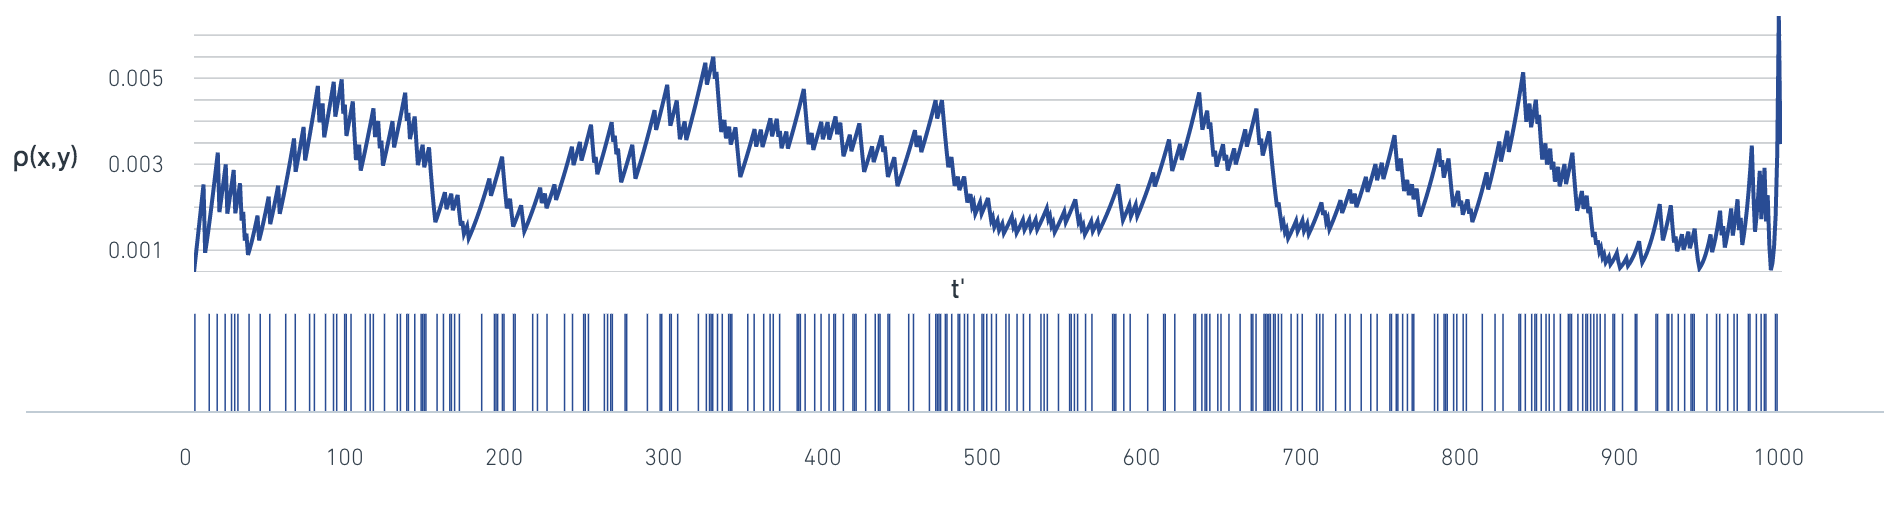
\includegraphics[width=\textwidth]{images/categorical_pearson}
%\caption[caption]{Pearson correlation coefficient\\
%For $p_1 = 20\%$, $p_2 = 30\%$, $t = 1000$, $t_1 = 350$, $t_1' \in [0, t]$}
%\label{fig:categorical_pearson}
%\end{figure}
%
%In Figure \ref{fig:categorical_pearson}, even a human could hardly give a better prediction in this case, as the separation between $C_1$ and $C_2$ is very blurry.
%Therefore, we used a Monte-Carlo method to get a better understanding of the accuracy of this metric. 
%\ref{fig:categorical_monte_carlo} shows the result of $n=5000$ random generations of $x$ and $y$ and displays the optimal $y_k$. Most of the distribution is centered around $t_1$, except for some mismatches for large values of $t_1'$, as in \ref{fig:categorical_pearson}. $5\%$ of the times the predicted value is close to $t$. With $50\%$ chances, the predicted value $t_1'^*$ is less than $4\%$ away from the real value $350$.
%
%% mean, median, std (389.2532, 354.0, 152.91886309334112)
%% 50 80 90 95 99 [37, 127, 239, 372, 636]
%
%\begin{figure}[ht]
%\centering
%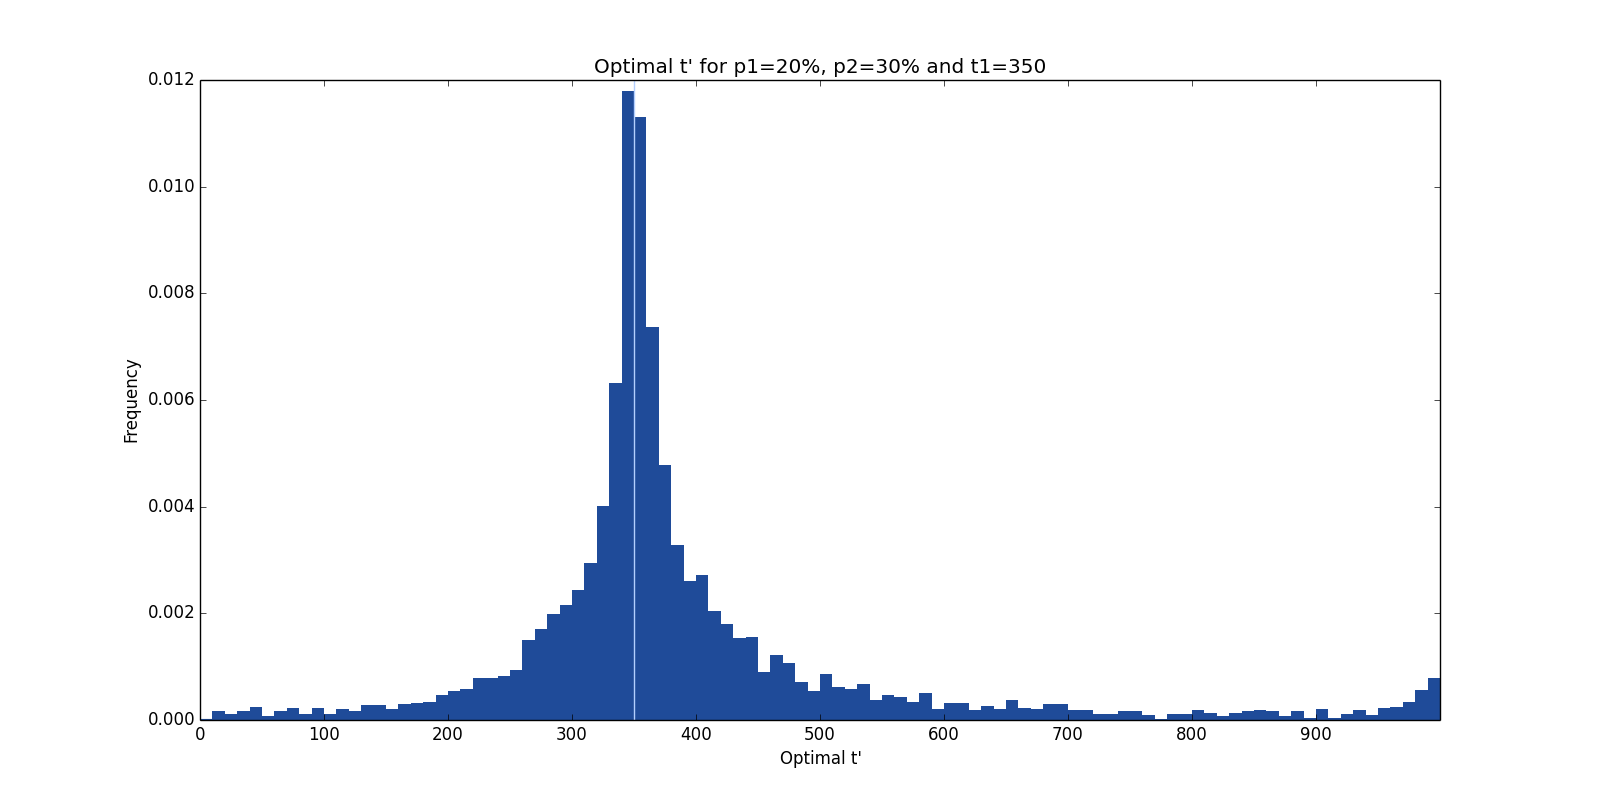
\includegraphics[width=\textwidth]{images/categorical_monte_carlo}
%\caption[caption]{Pearson correlation coefficient\\
%For $p_1 = 20\%$, $p_2 = 30\%$, $t = 1000$, $t_1 = 350$, $t_1' \in [0, t]$}
%\label{fig:categorical_monte_carlo}
%\end{figure}
%
%\paragraph{Numerical data}
%%TODO compute graph and set results here
%
%The correlation score will be quite low even when there is a high association, because the correlation is not linear. 
%While the series are correctly ranked, the value of the correlation is hard to interpret and does not indicate how significant the association is.
%
%
%
%
%\subsection{Spearman and Kendall Correlation Coefficients}
%
%Spearman and Kendall both defined correlation metrics based on the ranking of elements rather than their exact value. 
%
%The Spearman coefficient is the Pearson correlation between the ranks of the elements in $x$ and $y$, which for series with distinct elements is equivalent to:
%$$r_s = 1 - \dfrac{6 \sum_i (rank(x_i) - rank(y_i))}{t (t^2 - 1)}$$
%
%The Kendall coefficient computes the proportion of pairs $(i, j)$ for which both series have a concordant order $x_i > x_j$ or $x_i < x_j$:
%$$\tau = \dfrac{1}{t (t-1)}\sum_{i \neq j} sgn(x_i - x_j) sgn(y_i - y_j)$$
%
%\paragraph{Properties}
%
%While these two coefficients capture non-linear correlations, they still do not capture non-monotonous correlation, for instance if extreme values of $x$ (positive or negative) correspond to high values of $y$ (\textbf{P2.} $\nLeftarrow$ and \textbf{P3.} $\nLeftarrow$). 
%
%\paragraph{Categorical data}
%
%In the first case, Spearman and Kendall correlations are equivalent to Pearson correlation because both series can only take 2 different values, so sorting them gives the same result as taking their absolute value.
%
%\paragraph{Numerical data}
%In the second case however, these coefficients give different results than the Pearson coefficient. They can give better results because they capture non-linear correlations, but might miss the distinction between outliers and relatively high values.
%They will bias towards series that are impacted by few events, as they will consider the association to be perfect if the events $x$ correspond exactly to the largest values of $y$.
%
%These two coefficients are interesting to consider in addition to the Pearson coefficient as they capture other kinds of correlations, but they are also hard to interpret and could miss some obvious associations.
%
%\subsection{Null hypothesis}
%
%\paragraph{Properties}
%
%%TODO
%
%\paragraph{Categorical data}
%
%We can formulate the examples as null hypothesis problems.
%For the first example, the null hypothesis is:
%
%\vspace{1em}
%\medskip
%\noindent
%\fbox{
%    \parbox{\textwidth}{%
%    \vspace{-1em}
%\center $H_0$: Events in the time intervals $[0, t_1]$ and $[t_1, t]$ \\
%
%were drawn with the same probability $p$
%    }%
%}
%\medskip
%
%The z-test associated with this hypothesis is
%$$Z = \frac{p_1-p_2}{\sqrt{p(1-p)\left(\frac{1}{t_1}+\frac{1}{t_2}\right)}}$$
%
%We reject the null hypothesis if $Z > \alpha$. We note that $Z$ is proportional to the Pearson factor as $Z = \sqrt{t_{tot}}*\rho$. 
%
%\paragraph{Numerical data}
%For the second example, a hypothesis we could refute is that both groups (the values of $y$ when $x$ occurs and its values when $x$ does not occur) were drawn from the same distribution. This should give good results but requires a prior kind of distribution to be defined, in this case we can consider :
%
%\vspace{1em}
%\medskip
%\noindent
%\fbox{
%    \parbox{\textwidth}{%
%    \vspace{-1em}
%\center $H_0$: $y_{|x=1}$ and $y_{|x=0}$ were drawn from the same distribution $\mathcal{N}(\mu, \sigma)$
%    }%
%}
%\medskip
%
%The z-test associated with this hypothesis is
%$$Z = \frac{\mu_1-\mu_2}{\sigma}\sqrt{t_{tot}}$$
%
%where $\mu_1$ and $\mu_2$ are the average values of $y_{|x=1}$ and $y_{|x=0}$ respectively.\\
%
%In both cases, the null hypothesis definition requires a prior knowledge of the data, but gives us a good way to interpret the association score. For instance, when $Z > \alpha_{0.99}$, we can reject the null hypothesis with 99\% confidence, in other words the probability of occurrence if very likely to have changed at some point.
%
%\paragraph{Mutual Information}
%
%When considering categorical data, measures of association usually involve the information entropy. The metric that measures shared entropy is the mutual information. For categorical or discrete data, the mutual information is defined by
%
%$$I_{x,y} = H_x + H_y - H_{x, y} = \sum_i \sum_j p(x_i, y_j) \log \left( \dfrac{p(x_i, y_j)}{p(x_i) p(y_j)} \right)$$
%
%where $H$ denote the entropies and $p$ denotes probabilities. More specifically $p(x,y)$ is a joint probability function, and $p(x)$ and $p(y)$ are marginal probability distribution functions.
%
%Its definition can be generalized to continuous data (see \ref{appendix}):
%
%The mutual information is 
%$$I = H_1 + H_2 - H_{tot}$$
%where $H_{i} = -t_{i} \left(p_{i} \log p_{i} + (1-p_{i}) \log(1-p_{i})\right)$
%
%\paragraph{Properties}
%
%\paragraph{Categorical data}
%
%\paragraph{Numerical data}
%
%\subsection{Conclusion}
%
%%\begin{table}[]
%%\centering
%%\caption{My caption}
%%\label{my-label}
%%\begin{tabular}{lllll}
%%Metric                            & Properties &Categorical & Numerical & Interpretability & Generalizable \\
%%Pearson                         & No             & Yes            &                    & No                     & No \\
%%Spearman and Kendall & No             & Yes            &                    & No                     & No  \\
%%Null hypothesis             & Yes           & Yes            &                    & Yes                    & No \\
%%Mutual Information       & Yes           & Yes            &                    &                            & Yes
%%\end{tabular}
%%\end{table}
%
%
%
%
%\subsection*{Ranking candidate time series}
%
%%TODO Add
%\paragraph{Theory}
%Let's consider other candidate time series $y_i$ with value $C_1$ during $t_1'$ and $C_2$ during $t_2'=t_{tot}-t_1'$. 
%A good association metric should rank $y_i$ time series such that $y_{t_1}$ has the highest association with $x$. 
%In this example, all metrics studied here find the same optimal associated time series in theory, because $p_1'-p_2'$ decreases for values of $t_1'$ close to $t_2'$, and $\dfrac{1}{t_1'}$ or $\dfrac{1}{t_2'}$ is very large for extreme values of $t_1'$, so $z' < z$.
%
%\paragraph{Practice}
%In practice, we used the Monte-Carlo method to compute the error between the expected best candidate and the actual one. We note that results are pretty good, even for small differences between $p_1$ and $p_2$ where it's even hard for a human eye to detect the change in probability. The main bias is towards extreme values of $t_1'$, when the random samples had an unusually high (or low) frequency at the beginning or at the end. However, using the Null Hypothesis method we can ignore the best candidate when the hypothesis is rejected, in which increases the accuracy of the model.
%
%\chapter{Application to real data}
%
%\section{Preprocessing}
%
%%TODO Move to preprocessing
%\subsection*{Generalization}
%We can generalize the results above to any categorical data, and to events with any number of change of frequency. Using the null hypothesis, we can recursively split the event time series into phases where the frequency of occurrence is statistically constant. This can be used to preprocess event time series.
%The mutual information formula remains valid for any number of categories. It biases towards many categories, as the mutual information is always strictly positive. To balance this, we could penalize the mutual information such as defined in [A penalized mutual information criterion for blind separation of convolutive mixtures Mohammed El Rhabi, Guillaume Gelle, Hassan Fenniri, Georges Delaunay]. To keep our algorithm efficient enough to compare thousands of sub-second time series, we decided not to penalize the mutual information.
%
%\section{Data}
%
%\section{Results}
%
%\subsection{Discussion}
%
%Does not cover all faults, e.g. obvious ones are corrected, not significant. Helps for the hardest faults (recurrent + not systemmatic), both conception (quality) and in-service
%
%\chapter*{Conclusion}
%
%\newpage
%
%\appendix
%
%\chapter*{Appendix}
%\label{sec:appendix}
%\addcontentsline{toc}{section}{\nameref{sec:appendix}}
%
%\setcounter{section}{0}
%\renewcommand\thesection{\Alph{section}}
%\chapter{Mutual information generalization}\label{appendix}
%
%%TODO Mutual Info / Pearson-0Hyp correlation proofs
%
%We use Kraskov et al.'s idea \parencite{kraskov2004} to estimate the mutual information between numerical time series drawn from an unknown distribution. If we used the same definition as for discrete data, we would systematically have a mutual information of 1, because no pair of point would have exactly the same value, so the knowledge of a time series would enable us to know the value of the other one. However, this behavior is not expected, as learning these correlation 
%
%%TODO Define better the loss for time series, based on past values but using future value of the other one.
%
%The previous definition of mutual information was defined for categorical data. For numerical data, the joint probability of two variables is also well defined if the underlying distribution $\mu$ is known:
%
%$$MI = H(X) + H(Y) - H(X, Y)$$
%where $H(X) = \dfrac{1}{N}\sum\log\mu(x)$ and $H(X,Y) = \dfrac{1}{N^2}\sum\log\mu(x,y)$
%
%If the distribution is not known, it is still possible to approximate this underlying distribution by considering the $k$-nearest neighbors of each point. Given $k$, for each point $P$, we compute the distance $\varepsilon$ to its $k$-nearest neighbor. If the underlying distribution $\mu$ was uniform near $P$, then the probability of being in the ball of center $P$ and of diameter $\varepsilon$ would be:
%
%%TODO clarify
%$$\mathbb{P}(X \in \mathcal{B}(P, \varepsilon)) = \mu(P) \times c_d \varepsilon^d$$
%
%Where $ c_d$ is the volume of the unit ball $\mathcal{B}(0, 1)$.
%By deriving this expression, we get an approximation of the entropy:
%
%$$H(X) = -\psi(k) + \psi(N) + \log c_d + \dfrac{d}{N}\sum_{i=1}^{N}\log \varepsilon(i)$$
%
%And by extension of the mutual information between two numerical series. This expression is only valid for numerical data where all values are different (or at least where there are never more than $k-1$ elements with the same value), which can be circumvented by adding a small random noise.

%\end{document}
